\section{Methods}
\subsection{Problem formulation}
We represent the measurements available from each patient stay in a hospital as a regularly-spaced time series, unfolding in discrete timesteps indexed by integer $t \in \{1, 2, \ldots T\}$.
In later experiments, each timestep represents one hour.
In general, the length $T$ of each time series may vary across patient stays.

For each patient stay, we observe a sequence of feature vectors across time:
$\mathbf{x}_{1:T} = [\mathbf{x}_1, \ldots \mathbf{x}_T]$. 
The vector $\mathbf{x}_t$ represents a feature vector of possibly-missing-values of size $D$. Each index $d \in \{1, 2, \ldots D\}$ represents a specific \emph{measurement} (e.g. vital sign or lab test) of interest.
Entry $x_{td}$ represents either (i) the numerical value of measurement $d$ at time $t$, when available or (ii) a symbol $\textsc{NaN}$ indicating the intended vital or lab was not measured at time $t$.
Let $\mathbf{o}_{1:T} = \mathbf{o}_1, \ldots \mathbf{o}_T$ denote the set of indices of measurements that are observed (not missing) across all timesteps $1:T$.

%To represent realistic clinical data, the time series $\mathbf{x}_{1:T}$ must have 
%; our later experiments do assume a fixed $T=24$ hour period.

Each patient stay can be associated with a classification outcome $y$ taking one of 2 possible values (0 or 1) for binary classification or one of $C$ possible values, denoted $y \in \{1, 2, \ldots C\}$ for ordinal regression.
Adaptation of our methods to real-valued $y$ (aka regression) is straightforward conceptually; and in-fact has been shown to perform well in predicting soldier readiness from time-series of gait and stride sensory data \citep{rathSoldierReadiness}. Further illustration of evaluating PC-HMM regression models is left to future work.

Our goal is to build a probabilistic classifier %$h_{\theta}(\cdot)$ 
that can map any given feature time series $\mathbf{x}_{1:T}$ (which may have arbitrary missingness) to a probability vector over the $C$-classes of the outcome.
The training or learning problem is then how to optimize such a classifier given a finite training set.
We consider two distinct learning tasks, differing in assumptions about what training data is available.

\textbf{Supervised time-series classification with missingness.} 
For this task, we assume for model development we have access to a fully-labeled training dataset $\mathcal{D}^L$ of size $N$, where each element is a pair $(\mathbf{x}_{1:T}, y)$ representing the time series of measurements and corresponding class outcome.
In our target applications, each sequence $\mathbf{x}_{1:T}$ may have arbitrary missingness patterns during training or at prediction time on new patient stays.

\textbf{Semi-supervised time-series classification with missingness.}
For this task, we assume for model development we have access to both a (small) labeled training dataset $\mathcal{D}^L$ of size $N$ and a (large) unlabeled training set
$\mathcal{D}^U$ of size $M$.
Each element in $\mathcal{D}^L$ is a pair $(\mathbf{x}_{1:T}, y)$ of features and outcome representing one patient stay.
Each element in $\mathcal{D}^U$ is just the features $\mathbf{x}_{1:T}$ for a patient stay, without any known label. Again, we assume $\mathbf{x}_{1:T}$ might have arbitrary missingness when training or predicting.

\subsection{Model : Prediction Constrained HMMs for Semi-supervised Classification and Ordinal Regression}
Here, we review the HMM generative model, how its resulting belief-state vector representations can be used for prediction, and how prediction-constrained training can be used to balance discriminative and generative goals in settings with small labeled sets and feature missingness.

\textbf{HMM generative model.}
The HMM is defined by a fixed number of states $K$ (set as a hyperparameter), parameters governing \emph{transitions} (outgoing probability vectors for all $K$ states $\{ \pi_k \}_{k=1}^K$ and the initial state $\pi_0$) and \emph{emission} parameters $\{ \phi_k \}_{k=1}^K$.
Given $(\pi, \phi)$, the HMM defines a model for a sequence of regularly-spaced times of size $T$, where the random variables are the observable $D$-dimensional features over time $X \in \mathbb{R}^{T \times D}$ and the hidden discrete states $Z = [z_1, \ldots z_T]$.
The model
$p( X, Z | \pi, \phi)$ decomposes as
\begin{align}
	p( Z | \pi) = \text{Cat}( z_1 | \pi_0)
	\textstyle \prod_{t=2}^T \text{Cat}( z_t | \pi_{z_{t-1}} ),
	\quad 
	p( X | Z, \phi) = \textstyle \prod_{t,d} \mathcal{N}( x_{td} | \mu_{z_t,d}, \sigma_{z_t,d}^2 ).
 %\label{eq:logp_x_given_z_emission_likelihood}
\end{align}
In words, we draw $Z$ from a first-order Markov model, where each $z_t$ indicates one of the $K$ states.
Then, we generate each feature $x_{td}$ given $z_t$ via a state-specific emission model that \emph{factorizes} over feature dimensions $d$ and times $t$.
Elegantly, this factorization assumption allows exact computation of the marginal of observed features under \emph{any missingness pattern} (our specific model falls under the missing completely at random (MCAR) scenario since we do not explicitly assume that missingness depends on observed or unobserved data).
By applying the sum rule, the probability of the observed entries of $X$, denoted $X^{\mathcal{O}}$, given $Z$ is $\prod_{t,d \in \mathcal{O}} \mathcal{N}( x_{td} | \mu_{z_t,d}, \sigma_{z_t,d}^2 )$. Naturally, this factorization is a result of assuming independence between the $D$ input dimensions. We avoided estimating a full covariance matrix because when data is missing, estimating the parameters of a non-diagonal covariance matrix becomes more difficult and less reliable. The presence of missing data complicates the calculation of covariance since not all data points contribute to all parts of the covariance calculation. This can lead to biased or inaccurate estimates of the covariance parameters. Additionally, estimating the full covariance matrix increases the computational challenges.

\textbf{Computing beliefs.}
We can obtain useful representations from the HMM even though we never observe $Z$ by computing for each timestep $t$ and state $k$ the posterior belief of state occupancy: $b_{tk}(X^{\mathcal{O}} ) \triangleq p( z_t = k | X^{\mathcal{O}} )$.
Efficient dynamic programming achieves this in $O(TK^2)$ runtime. From an interpretability perspective, the beliefs provide information about the state of the patient at every time-point. In figure \ref{fig:interpretability_mortality} and \ref{fig:interpretability_los_prediction}, we show how the beliefs associated with 'risk' states are useful in providing interpretability at a patient-level and at a population level.

\textbf{Predicting binary outcomes from beliefs.}
Beliefs represent sufficient statistics for the HMM's latent state at each timestep, and thus could be useful representations for classification.
We condense all $T$ belief vectors into an average occupancy vector 
$\bar{b} = [\bar{b}_1, \ldots \bar{b}_K]$, where $\bar{b}_k = \frac{1}{T} \sum_{t=1}^T b_{tk}$.
We can then build a simple linear classification model:
\begin{align}
    p( y = 1 | X) = \sigma( \eta^T \bar{b}(X)) 
    \label{eq:binary_classification}
\end{align}
where $\eta \in \mathbb{R}^K$ are the weight parameters and $\sigma(r) = \frac{1}{1 + e^{-r}}$ is the logistic sigmoid function for real-valued inputs $r$. Besides average pooling, several alternative strategies have emerged in recent research as effective means to transform beliefs for downstream prediction. In the work by \cite{sotoodeh2019improving}, feature representations are derived by concatenating beliefs from the first and last time-points, enabling the capture of patient stay variability. Additionally,  \cite{hopePredictionConstrainedHiddenMarkov2021} demonstrate that applying a convolutional transformation to the belief sequence, followed by localized max pooling, leads to improved performance in human activity recognition tasks. 
While these alternative strategies exhibit promise, our own experiments focusing on mortality and length of stay prediction have conclusively shown that average pooling alone is sufficient to achieve competitive performance when compared to other baselines.

\textbf{Predicting ordinal outcomes from beliefs}
We wish to model the label $y \in \{1, \ldots, C\}$ given an $K$-dimensional feature vector $\bar{b}(x)$,
by
mapping features to a scalar location $g \in (-\infty, +\infty)$ on the real line via a generalized linear model $g(x) = \eta^\text{T} \bar{b}(x)$ with weights $\eta \in \mathbb{R}^K$.
A \emph{deterministic} model might then map this location to a class via a set of ordered thresholds $\theta_0 < \theta_1 < \ldots < \theta_C$:
\begin{align}
p( y = c | x) =     
    \begin{cases}
      1 & \text{if $\theta_{c-1} < g(x) \leq \theta_{c}$} \\
      0 & \text{otherwise}
    \end{cases} 
    \label{eq:deterministic_lik}
\end{align}
where we fix boundaries at $\theta_0 = -\infty$ and $\theta_C = +\infty$.
But the above would be flat almost everywhere as a function of parameters $\eta, \theta$, making gradient-based learning difficult. 

\emph{Cumulative link models} assume a smoother likelihood:
\begin{align}
p( y{=}c | x) = 
	H\left( \frac{\theta_c - g(x)}{\sigma_{scale}} \right) 
	- H\left( \frac{\theta_{c-1} - g(x)}{\sigma_{scale}} \right)
	\label{eq:ordinal_lik}
\end{align}
where $H$ is a cumulative distribution function (CDF) of a location-scale univariate distribution $\mathcal{H}$ over the reals, and $\sigma_{scale} > 0$ is a scale parameter.
Because $H$ as a CDF is a smooth increasing function according to Eq.~\eqref{eq:ordinal_lik}, increasing the value of $g$ gradually across any threshold $\theta_c$ leads to intuitively gradual changes in output probability (see Fig.~\ref{fig:clm_likelihood_vs_g}), not the sudden change across boundaries of Eq.~\eqref{eq:deterministic_lik}.

\begin{figure}[h!]
\begin{center}
\centerline{
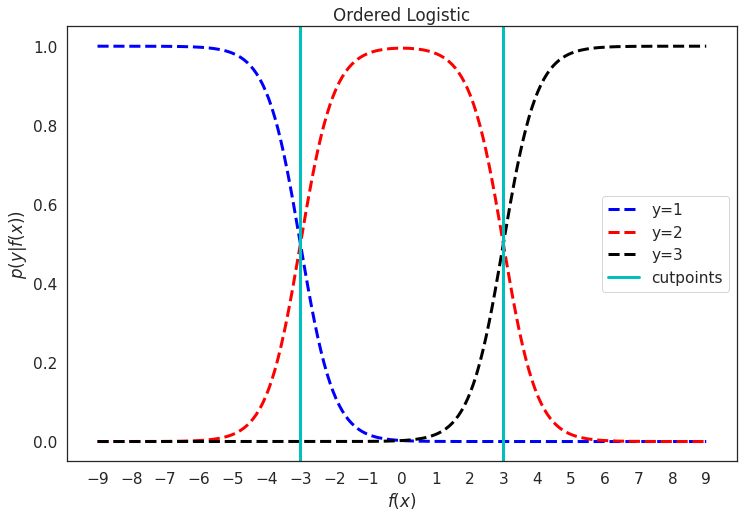
\includegraphics[width=0.8\textwidth]{content/chapters/semi_supervised_pchmm_missing_data/images/ordered_logistic.png}
}
\caption{Visualization of likelihood function for ordinal regression with 3 classes using the logistic distribution to simulate latent function noise}
\label{fig:clm_likelihood_vs_g}
\end{center}
\end{figure}

\textbf{Semi-supervised learning of HMMs via prediction-constrained training}

Now that our generative and discriminative model components are defined, we wish to \emph{estimate the parameters} of the model from a labeled training set $\mathcal{D}^L$ and an (optional) unlabeled set $\mathcal{D}^U$.

The first approach, simple and commonly used~\citep{sotoodeh2019improving}, is two-phase training that first fits standard HMM parameters $\pi, \mu, \sigma$ to all feature data (labeled and unlabeled), then fits the prediction parameters $\eta, \theta$ on the labeled set only.
\begin{align}
\text{phase 1:}~~
\hat{\pi}, \hat{\mu}, \hat{\sigma} &\gets \arg\max_{\pi, \mu, \sigma} \sum_{\xobs \in \mathcal{D}^L \cup \mathcal{D}^U} \log p( \xobs | \pi, \mu, \sigma ),
\label{eq:objective_two_stage}
\\ \notag 
\text{phase 2:}~~~~~
\hat{\eta}, \hat{\theta} &\gets \arg \max_{\eta, \theta} \sum_{\xobs, y ~\in \mathcal{D}^L} \log p( y | \xobs, \eta, \theta, \hat{\pi}, \hat{\mu}, \hat{\sigma}).
\end{align}
In phase 2, prediction parameters are estimated to maximize the label-given-feature likelihood, which is Eq.~\eqref{eq:binary_classification} for binary classification (where $\theta$ is unneeded) or Eq.~\eqref{eq:ordinal_lik} for ordinal regression.
Both objectives can be computed via HMM dynamic programming routines and are amenable to modern automatic differentiation, enabling estimating solutions via gradient descent algorithms.
For such algorithms, constrained parameters such as initial state probabilities \(\pi_0\), state transition probabilities \(\pi_k\), and Gaussian emission variances \(\sigma\) are reparameterized into the unconstrained real space so that all gradient updates yield valid parameters.
Phase 1 can also be solved with expectation-maximization~\citep{ghahramaniIntroductionHiddenMarkov2001b}.

The potential downside to the above approach is that the HMM is trained in an \emph{unsupervised} fashion. Class labels $y$ do not inform the values of $\pi, \mu, \sigma$.
Alternatively, we can maximize the joint supervised likelihood of features and any available labels: 
\begin{align}
    \pi, \mu, \sigma, \eta, \theta \gets
        \arg \max \sum_{\xobs, y \in \mathcal{D}^L}
            \log p( \xobs, y | \eta, \theta, \pi, \mu, \sigma) 
    + \sum_{\xobs \in \mathcal{D}^U}
    \log p( \xobs | \pi, \mu, \sigma)
\label{eq:objective_supervised_joint}
\end{align}
Again, both terms (and their gradients) can be computed in straightforward fashion, as in the two-stage method above.
The main issue with this approach is that while labels can inform the values of the HMM parameters $\pi, \mu, \sigma$, the objective does not encode our practical goal to prioritize predicting labels from features well even when we have few labels. 
This deficiency is reflected in our later results in Figure \ref{fig:mortality_prediction_results}, where this ``supervised'' approach to HMM training is hardly better than the two-stage unsupervised-then-predict method when we have few labels ($N \ll M$).

Recognizing the limitations of these methods, we arrive at our proposed \emph{prediction-constrained} (PC) objective, which directly encodes our goals: first and foremost, achieve label-from-feature prediction better than some threshold $\epsilon$, while also learning a good generative model if possible (to improve handling of missingness). Formally, we wish to estimate parameters by solving the constrained objective

\begin{align}
\pi, \mu, \sigma, \eta, \theta \gets \arg\max & \sum_{\xobs \in D^L \cup D^U} \log p(\xobs | \pi, \mu, \sigma) 
\label{eq:standard_pc_constrained},
\\ \notag
\text{subj. to:} \quad & 
\sum_{\xobs, y \in D^L} \log p(y | \xobs, \pi, \mu, \sigma, \eta, \theta) \geq \epsilon.
\end{align}

Directly handing the constraint here is difficult, so we transform the problem to be more amenable to modern gradient-based learning. 
By applying the theory of Langrange multipliers~\citep{bertsekasConstrainedOptLagrange1996}, we can form an equivalent unconstrained PC objective
\begin{align}
\pi, \mu, \sigma, \eta, \theta \gets \arg\max \sum_{\xobs \in D^L \cup D^U} \log p(\xobs | \pi, \mu, \sigma) 
+ ~~\lambda \sum_{\xobs, y \in D^L} \log p(y | \xobs, \pi, \mu, \sigma, \eta, \theta).
\label{eq:standard_pc_unconstrained}
\end{align}
For each tolerance $\epsilon$, there exists a scalar $\lambda > 0$  such that the maximizer of Eq.~\eqref{eq:standard_pc_unconstrained} 
is an optimum of Eq.~\eqref{eq:standard_pc_constrained}. 
Scalar $\lambda$ thus plays an analogous role as $\epsilon$ in the constrained objective; to achieve a higher prediction quality $\epsilon$, we would solve the above with a larger $\lambda$. 
In the special case of $\lambda = 1$, we recover the earlier supervised objective in Eq.~\eqref{eq:objective_supervised_joint}. 
We intend usually that $\lambda \gg 1$, which encourages better predictions of $y$ from $x$, trading off the quality of generative modeling of $x$ when necessary.


% \textbf{Prediction constrained training.} 
% Now that our generative and discriminative components are defined, we show how the prediction constrained framework is adapted to semi-supervised learning.
% We wish to fit the parameters of the HMM to a labeled dataset $\mathcal{D}^L$ containing many pairs of feature time-series $X$ and class label $y$ as well as an optional unlabeled dataset $\mathcal{D}^U$ containing only $X$ for many sequences.
% Prediction constrained training~\citep{hopePredictionConstrainedHiddenMarkov2021} aims to maximize generative performance but is unwilling to sacrifice prediction quality (the two aims are not treated equally).
% %seek an optimal fit for generating the time-series data (using the HMMs emission distribution($\phi$) to generate observations $x_n$ given a latent state, and the transition distribution($\pi$) to capture state transition at consecutive time-points), and simultaneously predict the labels $y_n$ (using beliefs from the HMM) accurately. 
% Our PC objective to minimize is
% \begin{align}
% %\resizebox{.6\hsize}{!}{$
% \mathcal{L}(\pi, \phi, \eta)
% \triangleq
% \sum_{X \in \mathcal{D}^L \cup \mathcal{D}^U}{{-}\log p( X^{\mathcal{O}} | \pi, \phi)}
% - \lambda 
% \sum_{X,y \in \mathcal{D}^L}{\log p(y|X, \pi, \phi, \eta)}
% %$}
% \end{align}

% The predictor distribution $p(y|X, \pi, \phi, \eta)$ is replaced by equation \ref{eq:binary_classification} or equation \ref{eq:ordinal_lik} for binary classification or ordinal regression respectively. To emphasize the classification task's importance, we set tradeoff parameter $\lambda \gg 1$, selecting its specific value via a validation set.

\textbf{PC-HMM Initialization}: We initialize the HMM's emission's parameters using K-means clustering. For ordinal regression, we initialize the emission's parameters for each class separately and then aggregate the learned clusters by retaining the states that are maximally distant from each other. We set the HMM's initial state probabilities to a uniform with probability $1/K$. For the transition distribution, we initialize such that self transitions probabilities (diagonal elements of the transition matrix) are 0.5, while the off-diagonal entries are $0.5/(K-1)$.We initialize the predictor weights by training a supervised model (logistic regression for binary classification or ordered logistic for ordinal regression) using the initial beliefs as features. We additionally apply L2 regularization on the predictor weights to prevent overfitting.


\subsection{Justifying Usage of The Prediction Constrained (PC) Framework}
The PC framework is built to model tasks containing both labelled and unlabelled examples. In case of time-series health record datasets, unlabelled examples include medical records (including vitals, lab measurements, medications etc.) of patient stays for whom outcome labels may not be available (for example, due to the high cost of obtaining clinician annotated disease labels). In contrast, labelled examples include medical records of patient stays for whom clinician annotated labels exist. The goal of the PC framework is to improve the predictive performance on labelled examples (over a fully supervised approach) by utilizing the unlabelled examples. This is done by maximizing the generative performance on both the labelled and unlabelled examples. While simultaneously adhering to performance constraints on the labelled set.

To formulate the core principle of the PC framework and highlight it's benefits, we first consider a more generic training approach,  \textit{regularized joint maximum likelihood optimization}. We consider a dataset $D$ containing labelled examples $D^L=\{x_n, y_n\}_{n=1:N^{L}}$ and unlabelled examples $D^{U}=\{x_n\}_{n=1:N^{U}}$. Additionally, we assume $h_n$ is a hidden variable, such that the generative process is as follows : (1) Generate $h_n$ from prior distribution parameterized by $\xi^h$; (2) Generate $x_n$ given $h_n$ from a distribution parameterized by $\xi^x$; (3) Generate $y_n$ given $x_n$ and $h_n$ parameterized by $\xi^y$. The joint distribution over $x_n, y_n, h_n$ is as follows :

\begin{align}
    p(x_n, y_n, h_n|\xi^h, \xi^x, \xi^y)=p(h_n|\xi^h)p(x_n|h_n, \xi^x)p(y_n|x_n, h_n, \xi^y)
\end{align}

Regularized maximum likelihood minimizes the following objective and obtains the optimal parameters $\xi^{ML}$.

\begin{align}
    \xi^{ML} = \min_{\xi=\{\xi^h, \xi^x, \xi^y\}} -\Sigma_n \log p(x_n, y_n|\xi) + R(\xi)
\end{align}
where $R(\xi)$ is the regularizer on the model parameters. 
The main issue with regularized maximum likelihood is that it assumes a symmetric relationship between $x_n$ and $y_n$. In other words, jointly maximizing the likelihood of $x_n$ and $y_n$ does not clearly highlight the practitioner's goal of predicting $y_n$ given $x_n$, rather than $x_n$ given $y_n$. To overcome this issue, the PC framework clearly specifies the need to learn a generative model for data $x$ that simultaneously achieves some threshold performance $\epsilon$ while predicting $y$ from $x$ with the following objective.
\begin{align}
\min_{\xi=\{\xi^h, \xi^x, \xi^y\}} \quad & -\Sigma_{n\in D^L \cup D^U} \log p(x_n|\xi^h, \xi^x) + R(\xi),
% \label{eq:standard_pc_constrained}
\\ \notag
\text{subj. to:} \quad & 
-\Sigma_{n\in D^L} \log p(y_n|\xi^h, \xi^x, \xi^y)\leq \epsilon
\end{align}

By applying the theory of Langrange multipliers, the unconstrained PC objective is :
\begin{align}
    \xi^{PC}=\min_{\xi=\{\xi^h, \xi^x, \xi^y\}} -\Sigma_{n\in D^L \cup D^U} \log p(x_n|\xi^h, \xi^x) - \lambda \Sigma_{n\in D^L} \log p(y_n|\xi^h, \xi^x, \xi^y) + R(\xi)
% \label{eq:standard_pc_unconstrained}
\end{align}
The PC objective clearly prioritizes predictions of $y_n$ from $x_n$ by setting $\lambda>1$ and eliminates the symmetric assumption between $x_n$ and $y_n$. 
This is also justified empirically in Figures \ref{fig:mortality_prediction_results} and \ref{fig:MIMIC_los_prediction_results}, where we see that models trained with the PC objective ($\lambda>>1$) always outperform models trained with maximum likelihood ($\lambda=1$, shown as supervised HMM), and models where the supervised and unsupervised components are trained separately in a 2 step process ($\lambda=0$, shown as unsupervised HMM $+$ predictor). In the following sub-sections, we show how the PC framework is applied to time-series data by choosing a HMM as the generative component. We further show how missing data can be handled elegantly without the need for imputation, and how missing labels can be handled via the semi-supervised extension of the PC framework for clinical prediction tasks involving binary classification as well as ordinal regression.

% \subsection{Baseline Semi-supervised learning adapted to Time-Series}

% Recent progress in improving deep classifiers in the SSL setting has been made under the family of \emph{consistency regularization}.
% Following the unified analysis in \citet{zhuRichGetRicher2022}, these approaches train a deep network $f_{\theta}$ with weights $\theta$ to minimize a two-term loss:

% \begin{align}
% \sum_{X, y \in \mathcal{D}^L }{\ell( y, f_{\theta}(X) )}
%  + \lambda \hspace{-6pt}
%  \sum_{X \in \mathcal{D}^U}{\ell( y'(X), f_{\theta}(X) )}
% \end{align}
% Here, $\ell(\cdot, \cdot)$ is a loss function, $\lambda > 0$ is a tradeoff hyperparameter, $y'(X)$ is a labeling transformation, and $a(\cdot)$ represents an (optional) data augmentation transformation.
% Below, we describe how both MixMatch and FixMatch fit this framework via concrete realizations of $y'$, $a$, and $\ell$.

% In practice, to minimize this loss via minibatch gradient descent we start $\lambda$ at zero for a few hundred epochs, and gradually ramp up to a small positive value over a few hundred more epochs.
% This ensures that early learning fits well to the labeled set, while letting the unlabeled set also influence results later on.

% \textbf{MixMatch for time series.}
% MixMatch~\citep{berthelotMixMatchHolisticApproach2019} is a recent state-of-the-art SSL algorithm based on two key ideas.
% First, smooth transitions between classes in feature space are desirable and achievable via an interpolating augmentation scheme known as MixUp~\citep{zhangMixupEmpiricalRisk2017}.
% Second, it is useful to ensure consistency in the predicted label across multiple augmentations of the same source features.
% Originally designed for images, it has recently been applied to time series  \citep{goschenhofer2021deep}.
% % to encourage smooth transitions between classes and encourages all augmentations of the same source features to lead to the same predictions.

% We set the labeling function $y'(X)$ to produce temperature-sharpened probability vectors averaged across multiple augmentations of examples X.
% The augmentation transformation $a(\cdot)$ uses MixUp to interpolate between labeled examples (see \citep{berthelotMixMatchHolisticApproach2019} for details).
% As a basic augmentation procedure applicable to time series, we add Gaussian noise $\mathcal{N}(0, \epsilon^2)$, following \citet{goschenhofer2021deep}, with standard deviation $\epsilon$ set to 0.1 and 1.
% For the backbone architecture $f_{\theta}$, we use a Gated Recurrent Unit(GRU)~\citep{gru_original}.

% \textbf{FixMatch for time series.}
% Similar to MixMatch, FixMatch~\citep{sohnFixMatchSimplifyingSemisupervised2020} is another recent state-of-the-art SSL algorithm based on consistency regularization and pseudo-labeling. Pseudo-labels for weakly augmented unlabeled examples are only retained if the model produces high-confidence predictions (we try 0.6 and 0.8 as thresholds for high confidence predictions). Consistency regularization and the augmentation procedure is the same as MixMatch. Again, we use GRU for the backbone architecture.

% \subsection{Baselines for Supervised Learning With Time-Series}
% \textbf{Gated Recurrent Unit with Decay (GRU-D)} GRU-D \citep{cheRecurrentNeuralNetworks2018} The GRU-D model is an adaptation of the standard GRU (Gated Recurrent Unit) architecture, tailored specifically for handling clinical time series data with missing values and irregular time intervals. GRU-D elegantly addresses the challenges of modeling clinical data by integrating information about missingness patterns and elapsed time between observations directly into the model.

% GRU-D extends the GRU by incorporating two main components: decay mechanisms for missing values and modeling elapsed time between observations.
% \begin{itemize}
%     \item Masking : GRU-D uses a masking mechanism to handle missing values. For each input feature, a binary mask (denoted as $m$ is used, which has a value of 1 if the feature is observed and 0 if it's missing. This mask is used to modulate the input and decay rates.
%     \item Decay Rate: This is a mechanism in GRU-D to capture the elapsed time between two consecutive observations. This decay rate ensures that the effect of a distant past observation decreases as time progresses.
% \end{itemize}

% The equations for GRU-D with the missing data handling and decay mechanisms can be described as:
% \begin{align*}
%     &\gamma_t = \text{tanh}(W_d \delta_t + b_d)\\
%     &h'_{t-1} = m_t \odot h_{t-1} + (1 - m_t) \odot (\gamma_t \odot h_{t-1})
% \end{align*}
% Where $\gamma_t$ is the decay rate, $\delta_t$ is the elapsed time since the last observation and $h'_{t-1}$ is the decayed previous hidden state.
% The decayed hidden state $h'_{t-1}$ replaces the regular $h_{t-1}$ in the GRU equations. $W_d$ and $b_d$ are learned parameters and $m_t$ represents the missingness mask (1 means observed, 0 means missing)

% The last hidden state is then passed through the fully connected layers to get the final classification output:
% \begin{align*}
%     \hat{y} = f_{out}(W_c h_T + b_c)
% \end{align*}
% Where $W_c$  and $b_c$ are trainable parameters of the fully connected layer. $h_T$ is the final hidden state from GRU-D.
% $f_{out}$ is the fully connected output layer.

% This output $\hat{y}$ is then used to compute the classification loss, using binary cross-entropy, which is then minimized during training.

% \textbf{Bidirectional Recurrent Imputation Time Series (BRITS)} BRITS \citep{caoBRITSBidirectionalRecurrent2018} is designed as a bidirectional RNN that performs imputation and classification/regression jointly in one neural graph. The hidden states are computed in both directions and concatenated to capture context from past and future time steps:
% \begin{align*}
%     &\overrightarrow{h}_t = \text{RNN}\left(\overrightarrow{h}_{t-1}, x_t\right) \tag{Forward RNN}\\
%     &\overleftarrow{h}_t = \text{RNN}\left(\overleftarrow{h}_{t+1}, x_t\right)
%     \tag{Backward RNN}\\
%     & h_t = [\overrightarrow{h}_t, \overleftarrow{h}_t]
%     \tag{combined hidden state}
% \end{align*}
% Finally, the sequence label $\hat{y}$ is predicted as 
% \[
% \hat{y} = f_{out}(\Sigma_{i=1}^T\alpha_i h_i)
% \]
% where $f_{out}$ is the output layer and $\alpha_i=1/T$.
% If a measurement $x_t$ at time $t$ is missing, it is replaced by a complement value $\hat{x_t}=W_x h_{t-1}+b_x$ where $W_x$ and $b_x$ are learned parameters. Additionally, the model incorporates a consistency loss to enforce the prediction in each step to be consistent in both directions. The consistency loss at time $t$ is given by $l_t^{cons}(\hat{x_t}, \hat{x_t'})=MAE(\hat{x_t}, \hat{x_t'})$, where $x_t$ is the estimated sequence in the forward direction and $\hat{x_t'}$ is the estimated sequence in the backward direction. The final loss $l$ is given by
% \begin{align*}
%     l = \Sigma_{t=1}^T l_t^{cons}(\hat{x_t}, \hat{x_t'}) + l_t^{imp}(x_t, \hat{x_t})+l^{BCE}(y, \hat{y})
% \end{align*}
% where $l_t^{cons}$ is the mean absolute error applied to the missing observations, $l_t^{imp}$ is the mean absolute error applied to the observed dimensions and $l^{BCE}$ is the binary cross entropy for classifying the output.

\subsection{Baseline neural nets for fully-supervised classification with missingness}
\label{sec:baselines_RNN}

We now consider alternative deep models intended to produce effective predictions for clinical time series, even with some missingness, but that can only make use of labeled datasets. These approaches cannot easily benefit from an extra large unlabeled dataset $\mathcal{D}^U$. We focus specifically on two methods in the recurrent neural net tradition that are both well-known and competitive: the Gated Recurrent Unit with Decay (GRU-D)~\citep{cheRecurrentNeuralNetworks2018} and Bidirectional Recurrent Imputation Time Series (BRITS)~\citep{caoBRITSBidirectionalRecurrent2018}, each summarized below.

\textbf{GRU-D : Gated recurrent Unit with decay model} \citep{cheRecurrentNeuralNetworks2018} developed the GRU-D to adapt the standard GRU (Gated Recurrent Unit) architecture by~\citep{gru_original} in order to specifically handle clinical time series data with missing values and long time delays between non-missing values. 
GRU-D extends the GRU by producing a complete feature vector at every time step, imputing any missing values between the last observation and a population mean via a  learnable, variable-specific decay mechanism informed by the time since last observation. Another similar decay mechanism informs the GRU-D's continuous-valued hidden state vector.
Ultimately, like any recurrent neural net, the GRU-D can be viewed as a deterministic mapping of input time series $\mathbf{X}$ of length $T$ to a representation vector $h_T$ at the final timestep. Following \citep{cheRecurrentNeuralNetworks2018}, a fully-connected output layer maps $h_T$ to probabilities over the $C$ possible classes. 

\textbf{BRITS : Bidirectional Recurrent Imputation Time Series model} \citep{caoBRITSBidirectionalRecurrent2018} designed BRITS as a bidirectional RNN that jointly performs imputation and classification/regression. It generates forward and backward hidden state representations, concatenates them into per-timestep representations $h_t$, and creates a sequence-level representation through mean pooling, followed by a fully-connected layer to produce class probabilities. The BRITS model handles missing data by using bidirectional recurrent neural networks that incorporate both past and future information, leveraging temporal correlations to impute missing values while considering the entire sequences, but its reliance on future data makes it unsuitable for real-time applications.

In our implementation, for both GRU-D and BRITS weight parameters are trained via gradient descent exclusively on the labeled training set $\mathcal{D}^L$ to minimize cross entropy. BRITS also includes a reconstruction and imputation consistency loss. For both methods, key hyperparameters like network size and learning rate settings are tuned on the validation set of each task. See table \ref{table: hyperparameters} for details.


\subsection{Baseline neural nets for semi-supervised time series classification without missingness}
\label{sec:baselines_SSL}

Many works have aimed to develop deep classifiers for SSL scenarios without abundant labeled data but plenty of unlabeled data. In this work, we focus on two strong baselines from the deep SSL literature, MixMatch~\citep{berthelotMixMatchHolisticApproach2019} and FixMatch~\citep{sohnFixMatchSimplifyingSemisupervised2020}. MixMatch recently delivered the most reliable accuracy gains (even over more recent methods) at a benchmark of self-supervised and semi-supervised methods for medical images \citep{huang2023accuracy}.
%of the SSL setting has been made under the family of \emph{consistency regularization}.
We adapt both methods to time series following \citep{goschenhofer2021deep}.
Importantly, neither method natively handles time series with arbitrary missingness. Thus, all methods here assume missing values have been filled by forward filling imputation (for all times after the first observation of channel $d$) or mean imputation (for all other times).
%fills in any missing values of any feature time series in any dataset.

Following the unified analysis of many SSL methods in \citep{zhuRichGetRicher2022}, these approaches train a deep network $f_{w}$ with weights $w$ to minimize a two-term loss:
\begin{align}
w^* \gets \arg\min \compactsum{X, y \in a(\mathcal{D}^L) }{\ell( y, f_{w}(X) )}
 + \lambda \hspace{-6pt}
 \compactsum{X \in a(\mathcal{D}^U)}{\ell^U( y'(X), f_{w}(X) )}
\end{align}
Here, $\ell(\cdot, \cdot)$ is a standard classification loss (e.g. binary cross entropy) and $\ell^U$ a corresponding unlabeled set loss, $\lambda > 0$ is a tradeoff hyperparameter, $y'(X)$ is a labeling transformation, and $a(\cdot)$ represents an (optional) data augmentation transformation. Below, we describe how both MixMatch and FixMatch fit this framework via distinct realizations of augmentations $a$ and loss $\ell^U$. 

Our implementation of both MixMatch and FixMatch uses a Gated Recurrent Unit (GRU)~\citep{gru_original} architecture to obtain a vector representation for the entire time series. 
We make predictions using representations from the last time step of each sequence.
For both methods, weights \( w \) are estimated using minibatch gradient descent with the Adam \citep{kingma2014adam} optimizer, starting with the unlabeled loss weight \( \lambda \) at zero and gradually increasing it \citep{tarvainen2017mean, berthelot2019mixmatch}. Key shared hyperparameters like \( \lambda \), GRU network size, and learning rate, as well as method-specific hyperparameters, are tuned on the validation set.

\textbf{MixMatch for time series.}
MixMatch is a semi-supervised learning algorithm that improves model performance by combining data augmentation, pseudo labels produced by the classifier, and a consistency loss to effectively utilize both labeled and unlabeled data. To adapt MixMatch \citep{berthelotMixMatchHolisticApproach2019} to time series, we follow Goschenhofer et al. \citep{goschenhofer2021deep}. For each input time series, we have all missing values imputed and then apply z-score transformations to standardize features.
Next, we apply two kinds of augmentation: add Gaussian noise \(\mathcal{N}(0, \epsilon^2)\) and apply MixUp \citep{zhangMixupEmpiricalRisk2017}, which interpolates between random pairs of features $\mathbf{X}$ and their labels (or pseudo labels) to create synthetic examples. We sample each pair's interpolation ratio from the distribution \(\text{Beta}(\alpha, \alpha)\). 
MixMatch defines loss $\ell^U$ to enforce label consistency between the model's prediction on an unlabeled instance and the average temperature-sharpened probability vector from several augmentations of that instance.
The key hyperparameters for MixMatch are scalars $\epsilon$ and $\alpha$. 



\textbf{FixMatch for time series.}
FixMatch \citep{sohnFixMatchSimplifyingSemisupervised2020} combines weak and strong augmentations to create diverse versions of unlabeled data, enabling the model to learn robust features by consistently predicting the same labels across these variations. Weak augmentations provide stable pseudo-labels, while strong augmentations introduce robustness by challenging the model with heavily altered data. To adapt FixMatch to time series, we add random Gaussian noise sampled from \(\mathcal{N}(0, 0.01)\) for weak augmentations and from \(\mathcal{N}(0, 1)\) for strong augmentations. Unlike \citep{goschenhofer2021deep}, who use RandAugment \citep{cubuk2020randaugment}, we only add Gaussian noise since time and magnitude warping hurt performance in our experiments. Pseudo-labels for weakly augmented examples are retained if the model produces high-confidence predictions, with thresholds of 0.6 and 0.8 explored. FixMatch's unlabeled loss $\ell^U$ uses these pseudo-labels as targets for strongly augmented versions of the same examples, ensuring consistent predictions across augmentations and leveraging high-confidence predictions to enhance model robustness and generalization.


\subsection{Justification of the $O(TK^2)$ belief computation runtime for HMMs}

The complexity largely stems from the number of states and the transitions between these states considered over the length of the observation sequence in an algorithm termed as Forward Backward Algorithm.

The forward algorithm computes the probability of observing the sequence up to time \( t \) and being in state \( k \). This is known as the forward probability, denoted as \( \alpha_t(k) \). The recursion formula for \( \alpha_t(k) \) is given by:

\[
\alpha_t(k) = \left( \sum_{j=1}^K \alpha_{t-1}(j) a_{jk} \right) b_k(o_t)
\]

Where:
\begin{itemize}
    \item \( \alpha_{t-1}(j) \) is the forward probability of being in state \( j \) at time \( t-1 \).
    \item \( a_{jk} \) is the transition probability from state \( j \) to state \( k \).
    \item \( b_k(o_t) \) is the probability of observing \( o_t \) given state \( k \) (the emission probability).
\end{itemize}


Computational Steps:
\begin{itemize}
    \item For each state \( k \) at each time \( t \), calculate \( \alpha_t(k) \).
    \item For each \( k \), the sum is over all \( K \) possible states \( j \), requiring \( K \) multiplications and \( K-1 \) additions.
    \item Thus, for each \( k \) and each \( t \), the computation is \( O(K) \).
    \item Since there are \( K \) states to consider at each time step, the complexity for each \( t \) is \( O(K^2) \).
\end{itemize}


Similarly, the backward algorithm computes the probability of the future observations given state \( k \) at time \( t \). This is known as the backward probability, denoted as \( \beta_t(k) \). The recursion formula for \( \beta_t(k) \) is given by:

\[
\beta_t(k) = \sum_{j=1}^K a_{kj} b_j(o_{t+1}) \beta_{t+1}(j)
\]

Where:
\begin{itemize}
    \item \( \beta_{t+1}(j) \) is the backward probability at state \( j \) at time \( t+1 \).
    \item \( a_{kj} \) is the transition probability from state \( k \) to state \( j \).
    \item \( b_j(o_{t+1}) \) is the emission probability at state \( j \) for observation \( o_{t+1} \).
\end{itemize}

Since both the forward and backward algorithms require \( O(K^2) \) operations at each of the \( T \) time steps, the overall computational complexity for running either algorithm is \( O(TK^2) \). This describes the amount of computational work needed to process an entire sequence with respect to the number of states and the length of the sequence, making clear the impact of the state space size and the sequence length on the computational demand.